% Supplement 1 -- generated from supplementary.md by md2optica.py
\documentclass[10pt]{article}
\usepackage[margin=2.5cm]{geometry}
\usepackage{graphicx,amsmath,url,caption}
\usepackage[T1]{fontenc}
\usepackage[utf8]{inputenc}
\title{Supplement 1:\\Practical Saturation of Freeform Microlens Arrays on Extended OLED Emitters and Design Routes beyond Lens Shape}
\author{}
\date{}
\begin{document}
\maketitle
\sloppy


Practical Saturation of Freeform Microlens Arrays on Extended OLED Emitters
and Design Routes beyond Lens Shape

This supplement collects the material that supports the main text but is not needed to follow its argument. It covers platform and campaign settings, statistical controls, normalization checks, convergence and cost calibrations, the recycling model, and the separately constrained asymmetric study. Notes S1–S8 follow the order in which the main text cites them. Main-text references are cited as "main ref. n".

\section*{Note S1 | Common platform and campaign settings}

All simulations share one source model, one substrate, and one textured patch size. Table S1 lists the common platform. Table S2 lists every setting that differs between campaigns. Anything not listed is identical across campaigns.

\begin{table}[htbp]
\centering
\footnotesize
\caption*{Table S1. Common platform.}
\begin{tabular}{p{0.16\linewidth}p{0.80\linewidth}}
\hline
Quantity & Value \\
\hline
Source & disc, radius 1 mm, CPS microcavity dipole distribution $I_{\mathrm{sub}}(\theta,\lambda)$ \\
Substrate & thickness $d_{\mathrm{sub}} = 1.295$ mm, $n = 1.51$ \\
Textured patch & 25 \ensuremath{\times} 25 mm (all campaigns; see Note S3) \\
Lenslet & \ensuremath{\sim}10 \ensuremath{\mu}m radius, hexagonal placement (X 0.0866 mm, Y 0.1 mm) \\
Lens material & N-BK7, $n = 1.517$ at 589 nm, index-matched to the substrate, identical for every lens class and family \\
Emission window & 453–753 nm \\
Emitter & $\eta_{\mathrm{rad}} = 0.98$, horizontal dipole ratio 0.865 \\
Stack & Al / ETL / EML / HTL / ITO / glass, ETL and HTL thicknesses free in 10–150 nm \\
Shape parameterization & 7 spline control points, endpoints fixed at (0,1) and (1,0); five free points give 10 shape variables with $x_2 \ldots x_6$ constrained monotonic \\
Design vector & 13 variables = 10 shape + $d_{\mathrm{ETL}}$ + $d_{\mathrm{HTL}}$ + stretch$_Z$ \\
\hline
\end{tabular}
\end{table}

Angular bands are polar bins of the far field over the full azimuth: 0–20\ensuremath{^\circ}, 20–40\ensuremath{^\circ}, 40–60\ensuremath{^\circ}, and 60–80\ensuremath{^\circ}. The band selectivity is $S_j = \mathrm{EQE}_{j}/\mathrm{EQE}_{\mathrm{total}}$. The Lambertian partition, $S_j^{\mathrm{Lam}} = \sin^2\theta_{\mathrm{hi}} - \sin^2\theta_{\mathrm{lo}}$, gives 0.117 / 0.296 / 0.337 / 0.220.

\begin{table}[htbp]
\centering
\footnotesize
\caption*{Table S2. Per-campaign settings.}
\resizebox{\linewidth}{!}{\begin{tabular}{llllll}
\hline
Campaign & Script & Free variables & Search budget & Search fidelity & Final fidelity \\
\hline
Convex, weighted sweep & \texttt{pareto\_front\_freeform.m} & 13 & 150 random + 120/weight + 15 polish, $w \in \{0,\,0.25,\,0.5,\,0.75,\,1\}$ & 10,000 rays, 31 \ensuremath{\lambda} & 50,000 rays, 151 \ensuremath{\lambda}, \ensuremath{\times}3 \\
Convex, per-band & \texttt{opt\_4band\_freeform.m} & 13 & 60 + 15 polish per arm, 5 arms & 10,000 rays, 31 \ensuremath{\lambda} & 50,000 rays, 151 \ensuremath{\lambda}, \ensuremath{\times}3 \\
Convex, total EQE only & \texttt{freeform\_EQEtotal.m} & 13 & 140 per start, 3 independent starts & 10,000 rays, 31 \ensuremath{\lambda} & 50,000 rays, 151 \ensuremath{\lambda}, \ensuremath{\times}3 \\
Restart control & \texttt{warmstart\_from\_hemisphere.m} & 13 & 40 + 15 + 15 polish per arm, 5 arms & 10,000 rays, 31 \ensuremath{\lambda} & 50,000 rays, 151 \ensuremath{\lambda}, \ensuremath{\times}3 \\
Hemispherical reference & \texttt{opt\_hemisphere\_arms.m} & 3 (cavity + height) & 30 + 10 polish per arm, 5 arms & 10,000 rays, 31 \ensuremath{\lambda} & 50,000 rays, 151 \ensuremath{\lambda}, \ensuremath{\times}3 \\
Inverted (concave) & \texttt{opt\_4band\_inverted.m} & 13 & 60 + 15 polish per arm, 4 arms & 10,000 rays, 31 \ensuremath{\lambda} & 50,000 rays, 151 \ensuremath{\lambda}, \ensuremath{\times}3 \\
Randomly assembled & \texttt{stress\_random\_mla.m} & 6 assembly statistics & 50 random + 60 + 15 polish & 5,000 rays, 16 \ensuremath{\lambda} & 10,000 rays, 151 \ensuremath{\lambda}, \ensuremath{\times}3 seeds \\
Convergence check & \texttt{convergence\_check.m} & re-evaluation only & 20 designs & — & 200,000 rays \ensuremath{\times}3; 450–750 nm broadband \\
Patch-size check & \texttt{check\_patch\_convergence.m} & re-evaluation only & 1 design \ensuremath{\times} 4 patch sizes & — & 50,000 rays, 151 \ensuremath{\lambda} \\
20–40\ensuremath{^\circ} confirmation & \texttt{reeval\_confirm\_2040.m} & re-evaluation only & 2 designs \ensuremath{\times} 5 repeats & — & 50,000 rays, 151 \ensuremath{\lambda} \\
\hline
\end{tabular}}
\end{table}

The inverted family uses a model file identical to the convex one except for the texture relief setting (\texttt{LibraryElementUnitCell.Bumps}, "Yes" \ensuremath{\rightarrow} "No"). The two families therefore differ in construction and nothing else. The randomly assembled family is the only campaign with reduced sampling (Note S6).

\section*{Note S2 | Hemispherical benchmark and restart control}

\textbf{Table S3} lists the entries behind $G_j$ in main-text Fig. 2b. Every entry comes from a fixed-patch (25 \ensuremath{\times} 25 mm) campaign, so the two columns share one normalization.

\begin{table}[htbp]
\centering
\footnotesize
\caption*{Table S3. Relative gain of the freeform optimum over the equally optimized hemisphere.}
\resizebox{\linewidth}{!}{\begin{tabular}{lllll}
\hline
Objective & freeform & hemisphere & $G_j$ & source of freeform entry \\
\hline
0–20\ensuremath{^\circ} & 0.06699 & 0.06682 & 1.003 & restart control \\
20–40\ensuremath{^\circ} & 0.16628 & 0.16591 & 1.002 & restart control \\
40–60\ensuremath{^\circ} & 0.19802 & 0.18503 & 1.070 & per-band campaign \\
60–80\ensuremath{^\circ} & 0.14075 & 0.13589 & 1.036 & restart control \\
total EQE & 0.5539 & 0.54679 & 1.013 & dedicated total-EQE campaign \\
\hline
\end{tabular}}
\end{table}

Each freeform entry is the better of the matched freeform campaigns. In the 40–60\ensuremath{^\circ} arm the restart control did not surpass the per-band optimum (0.19355 against 0.19802). In the 60–80\ensuremath{^\circ} arm it did (0.14075 against 0.13863). The total is from the dedicated campaign (0.5495 / 0.5530 / 0.5539 over three starts), and the restart control's same-session value of 0.5523 confirms it to within 0.3\%.

\textbf{Why the restart control was needed.} In the original per-band campaign, which was randomly seeded, the 0–20\ensuremath{^\circ} and 20–40\ensuremath{^\circ} gains came out below unity, at 0.946 and 0.966. Because the hemisphere is a point of the 13-variable feasible set, $G_j \ge 1$ holds for an exhaustive search. A value below unity is therefore a statement about the search, not about optics. It was also the strongest objection to the main result: a search that fails to recover a solution it contains cannot be trusted when it reports that nothing better exists. The restart control removes this ambiguity.

\textbf{Protocol.} Each arm's search restarts at that arm's hemispherical optimum: the fixed quarter-circle control points with that arm's optimized cavity thicknesses and lens height. The hemisphere point and eight perturbations within 8\% of each variable's range form the seed set. The search runs three ways: \texttt{surrogateopt} from the seed set, \texttt{patternsearch} from the surrogate winner, and \texttt{patternsearch} launched directly from the hemisphere point. The last is the most direct test of whether the hemisphere is a local optimum in thirteen dimensions. The winner is re-evaluated at final fidelity. The hemisphere baseline is re-measured in the same session at final fidelity. The archived value serves only as a cross-check. An arm counts as improved when the difference exceeds the pooled one-sided 95\% $t$ value at $2(N_{\mathrm{rep}}-1) = 4$ degrees of freedom, 2.13.

\begin{table}[htbp]
\centering
\footnotesize
\caption*{Table S4. Restart control.}
\resizebox{\linewidth}{!}{\begin{tabular}{llllllll}
\hline
Arm & hemisphere (archived) & hemisphere (re-measured) & dev. & restarted & gain & $t$ & winning branch \\
\hline
0–20\ensuremath{^\circ} & 0.06682 & 0.06677 \ensuremath{\pm} 0.00017 & 0.07\% & 0.06699 \ensuremath{\pm} 0.00013 & +0.32\% & 1.7 & polish from hemisphere \\
20–40\ensuremath{^\circ} & 0.16591 & 0.16595 \ensuremath{\pm} 0.00017 & 0.02\% & 0.16628 \ensuremath{\pm} 0.00020 & +0.20\% \ensuremath{\ddagger} & 2.1 \ensuremath{\ddagger} & surrogateopt \\
40–60\ensuremath{^\circ} & 0.18503 & 0.18486 \ensuremath{\pm} 0.00008 & 0.09\% & 0.19355 \ensuremath{\pm} 0.00010 & \textbf{+4.70\%} & \textbf{114.6} & polish from surrogate \\
60–80\ensuremath{^\circ} & 0.13589 & 0.13581 \ensuremath{\pm} 0.00014 & 0.06\% & 0.14075 \ensuremath{\pm} 0.00025 & \textbf{+3.64\%} & \textbf{29.6} & surrogateopt \\
total EQE & 0.54679 & 0.54679 \ensuremath{\pm} 0.00013 & 0.00\% & 0.55231 \ensuremath{\pm} 0.00004 & \textbf{+1.01\%} & \textbf{68.7} & polish from surrogate \\
\hline
\end{tabular}}
\end{table}

Uncertainties are the standard deviation over three high-precision repeats.

\ensuremath{\ddagger} The 20–40\ensuremath{^\circ} arm was the only borderline case. It was settled by re-measuring both stored designs with five fresh repeats each, with the search excluded. This gives hemisphere 0.16583 \ensuremath{\pm} 0.00015 against restarted 0.16631 \ensuremath{\pm} 0.00021, a residue of +0.29\% at $t = 4.1$ (five-repeat threshold 1.86). The residue is statistically real but three tenths of a percent in size.

\textbf{Reading the control.} The control is one-sided: the hemisphere is among the screened candidates, so the result cannot fall meaningfully below it. It is also biased toward reporting a gain, because the winner is the maximum over roughly seventy noisy search evaluations per arm. The near-zero outcomes are therefore conservative. The two groups differ in scale: residues of +0.29\% to +0.32\%, against margins of +1.01\% to +4.70\% at $t = 30$ to 115. This separation shows that the residues reflect an essentially absent margin rather than a weak search. In the 60–80\ensuremath{^\circ} arm the restart also beat the original campaign's own optimum, so starting at the hemisphere is simply a better search protocol in this design space. The two original sub-unity values were a search artifact, and the corrected values are 1.003 and 1.002.

\begin{figure}[htbp]
\centering
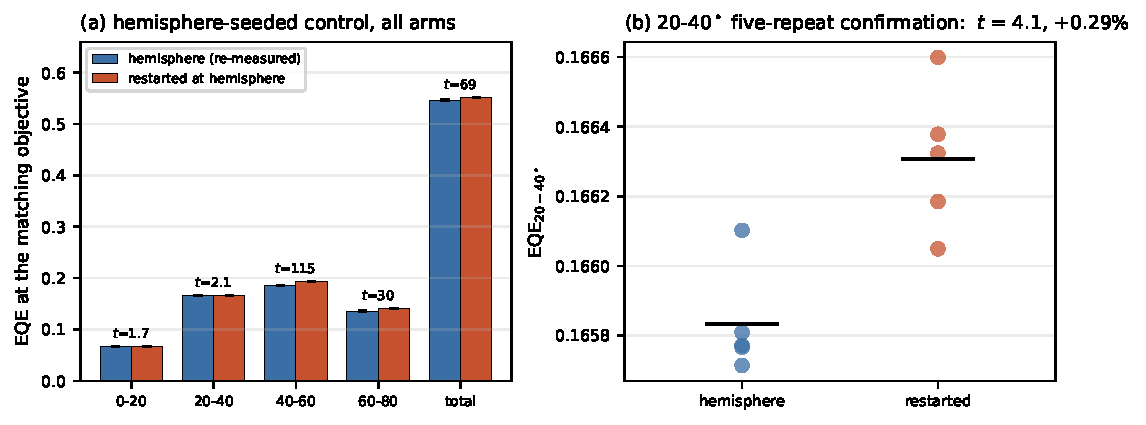
\includegraphics[width=\linewidth]{figures/figS1_restart_control.pdf}
\caption*{\textbf{Fig. S1.} \textbf{Restart control.} (a) Hemisphere baseline (re-measured in the same session) and restarted optimum for every arm, with standard deviations over three repeats and the $t$ value of each difference. (b) Five-repeat confirmation of the 20–40\ensuremath{^\circ} arm: individual repeats and means for both designs ($t = 4.1$, +0.29\%).}
\end{figure}

\section*{Note S3 | Patch-size dependence and normalization}

One fixed high-efficiency design, the weighted-sweep optimum at $w = 0.75$, was re-evaluated at final fidelity (50,000 rays, 151 \ensuremath{\lambda}) with only the textured patch size varied. The 15/25/35 mm rows are 3 repeats (\texttt{patch\_convergence\_result.mat}). The 100 mm row is 2 repeats from a follow-up run (\texttt{patch\_convergence\_100.mat}).

\begin{table}[htbp]
\centering
\footnotesize
\caption*{Table S5. Patch-size dependence.}
\resizebox{\linewidth}{!}{\begin{tabular}{lllll}
\hline
Patch (mm) & total EQE & s.d. & vs 25 mm & selectivity (0–20 / 20–40 / 40–60 / 60–80) \\
\hline
15 \ensuremath{\times} 15 & 0.51681 & 0.00016 & -4.79\% & 0.108 / 0.283 / 0.346 / 0.233 \\
25 \ensuremath{\times} 25 & 0.54282 & 0.00008 & — & 0.106 / 0.280 / 0.346 / 0.238 \\
35 \ensuremath{\times} 35 & 0.55128 & 0.00003 & +1.56\% & 0.106 / 0.279 / 0.346 / 0.239 \\
100 \ensuremath{\times} 100 & 0.5636 & 0.00003 & +3.83\% & 0.106 / 0.277 / 0.347 / 0.240 \\
\hline
\end{tabular}}
\end{table}

Three observations follow.

\begin{enumerate}

\item The initial rise saturates with a decay length of about 9 mm, four critical-angle round trips of 2.32 mm each. The far tail does not saturate. Between 35 and 100 mm the total still gains 2.2\%, about three times what a single exponential fitted to the first three points would allow. Light that is recycled many times migrates laterally over many tens of round trips before escaping. The total EQE of a finite film therefore increases slowly with its extent, and the 25 mm value is a lower bound, 3.7\% below the 100 mm value.

\item The angular composition is converged with respect to patch size. While the total gains 3.8\% from 25 to 100 mm, no band selectivity changes by more than 0.24 pp (0.11 pp between 25 and 35 mm). All ratios, correlations, and class comparisons are evaluated at equal patch and are unaffected.

\item The weighted-sweep campaign's archived best total, 0.5556, falls between the 35 mm and 100 mm values of the same design, while the design re-measures at 0.5428 on the 25 mm patch. That campaign's absolute normalization therefore corresponds to a larger effective patch. Its absolute totals are excluded from the $G_j$ comparison (Table S3). Its compositions and correlations, being ratios, are used. Its coarse-fidelity log maximum (0.5591 at 10,000 rays) is not used anywhere.

\end{enumerate}

\begin{figure}[htbp]
\centering
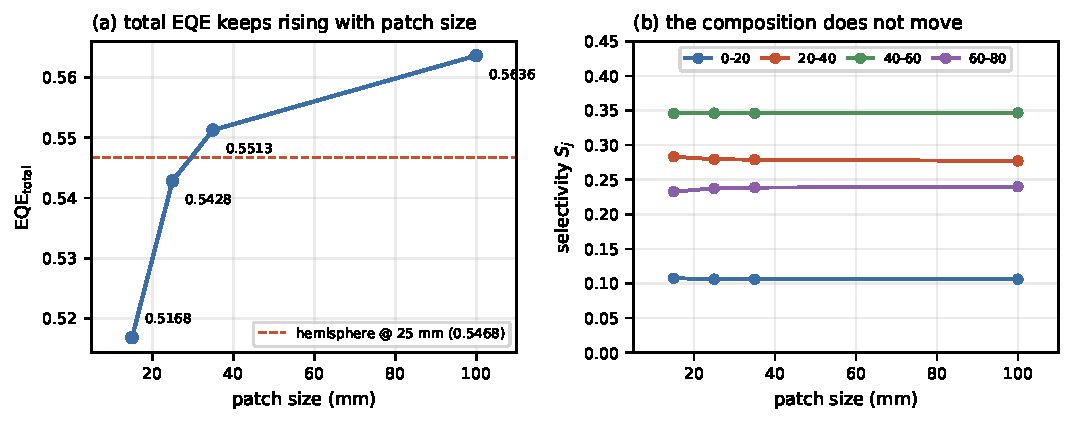
\includegraphics[width=\linewidth]{figures/figS2_patch_dependence.pdf}
\caption*{\textbf{Fig. S2.} \textbf{Patch-size dependence.} (a) Total EQE of one fixed design versus textured patch size, with the hemisphere baseline at 25 mm for scale. (b) Band selectivity of the same design versus patch size: the composition does not move.}
\end{figure}

\section*{Note S4 | Angular-composition statistics}

\textbf{Natural composition.} The natural composition is the median selectivity of the twenty designs with the highest total EQE in a campaign log. For the convex weighted-sum log it is 0.094 / 0.278 / 0.361 / 0.236. The 10–90\% spreads are 0.092–0.096, 0.277–0.281, 0.358–0.364, and 0.233–0.238.

\textbf{Dedicated versus natural.} The band-dedicated optima of the per-band campaign reach selectivities of 0.119 / 0.300 / 0.364 / 0.283. These are +27\%, +8\%, +1\%, and +20\% above the natural medians. The same designs lose total EQE: 3\%, 2\%, 1\%, and 11\% below that campaign's best total of 0.548. The net band-power gain is the product of the selectivity gain and the total-EQE ratio: 1.22, 1.05, 1.00, and 1.07 (Fig. S3). A stricter benchmark compares each dedicated optimum with the best value of the same band reached incidentally while another band was being optimized. Against that benchmark the dedicated optima win by only 6.3\%, 0.6\%, 4.5\%, and 5.8\%.

\begin{figure}[htbp]
\centering
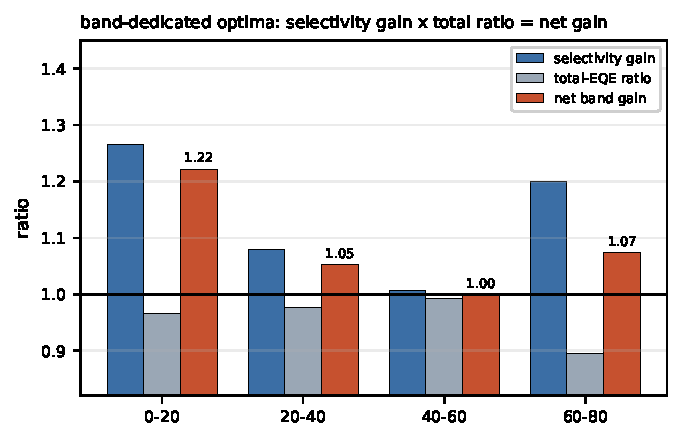
\includegraphics[width=\linewidth]{figures/figS3_gain_decomposition.pdf}
\caption*{\textbf{Fig. S3.} \textbf{Gain decomposition of the band-dedicated optima.} Selectivity gain $S_{\mathrm{win}}/S_{\mathrm{nat}}$, total-EQE ratio $E_{\mathrm{win}}/E_{\max}$, and their product, the net band-power gain (labelled).}
\end{figure}

\textbf{Selectivity across the design space.} Fig. S4 shows the four bands separately, over all 606 usable evaluations of the weighted-sum campaign. The log holds 691 evaluations. The remaining 85 traces failed to return a positive total EQE. The correlations between total EQE and $S_j$ are +0.60, +0.55, -0.12, and -0.57.

\textbf{Band ordering.} The tilt toward lower polar angles does not reorder the bands among efficient designs:

\begin{itemize}
\item In all 520 designs with total EQE \ensuremath{\geq} 0.40, the 40–60\ensuremath{^\circ} band carries the largest share.
\item Among the 421 designs with total EQE \ensuremath{\geq} 0.50, 416 follow the order 40–60\ensuremath{^\circ} > 20–40\ensuremath{^\circ} > 60–80\ensuremath{^\circ} > 0–20\ensuremath{^\circ}.
\item The 60–80\ensuremath{^\circ} band is the largest in 8 of the 606 designs, all with total EQE \ensuremath{\leq} 0.354.
\item The 60–80\ensuremath{^\circ} share exceeds the 20–40\ensuremath{^\circ} share in 85 of the 606 designs (14\%). Of these, 50 have total EQE < 0.40 and only 5 have total EQE \ensuremath{\geq} 0.50; these 5 are the exceptions to the full ordering above.
\end{itemize}

The same count in the other logs follows. The 40–60\ensuremath{^\circ} band is the largest in 100\% of the convex per-band designs, 99.4\% of the concave designs, and 100\% of the randomly assembled designs. The 60–80\ensuremath{^\circ} share exceeds the 20–40\ensuremath{^\circ} share in 19.2\%, 28.8\%, and 4.6\% of them, respectively.

\begin{figure}[htbp]
\centering
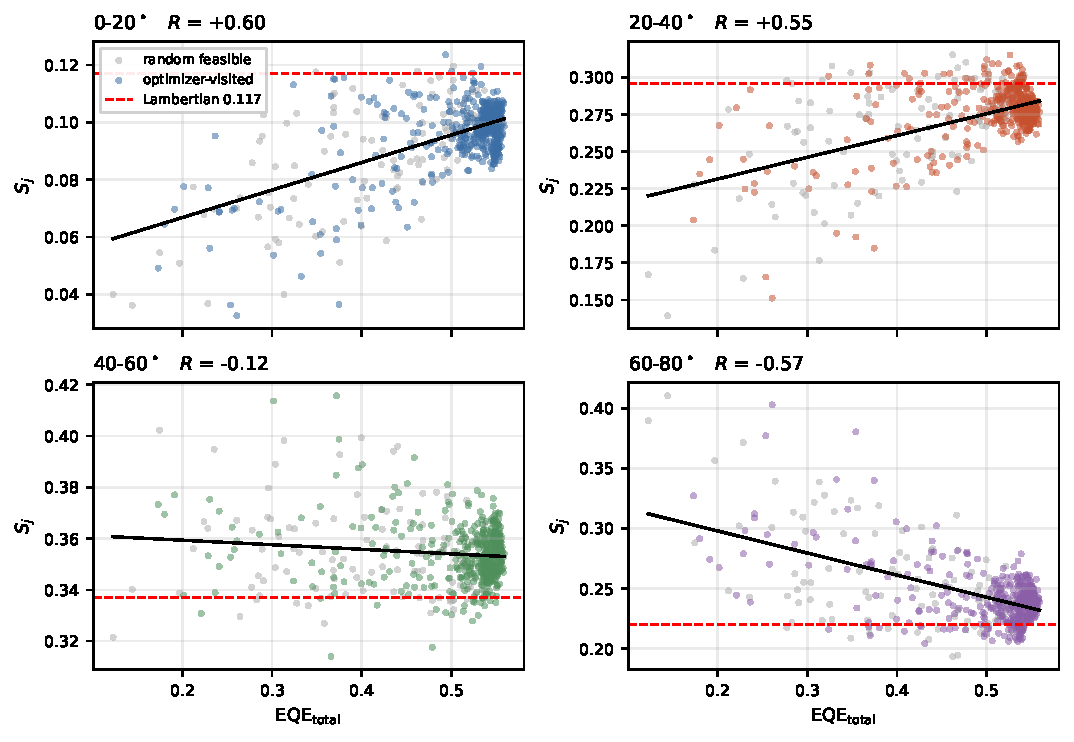
\includegraphics[width=\linewidth]{figures/figS4_selectivity_map.pdf}
\caption*{\textbf{Fig. S4.} \textbf{Band selectivity across the design space.} $S_j$ versus total EQE over all 606 usable evaluations of the weighted-sum campaign, separated into random feasible designs (grey) and optimizer-visited designs (colored), one panel per band. Black lines are least-squares fits; red dashed lines mark the Lambertian partition. Each vertical axis spans only a few percentage points.}
\end{figure}

\textbf{Family comparison.} Two statistics are given for each family, both computed from the family's own log: the top-twenty median and the population mean over every usable evaluation. Both are needed. The gap between them within one family is comparable to the gap between families under either statistic. A table with only one statistic would suggest family differences that the data do not support.

\begin{table}[htbp]
\centering
\footnotesize
\caption*{Table S6. Family comparison.}
\resizebox{\linewidth}{!}{\begin{tabular}{llll}
\hline
Family & best total EQE & top-20 median (0–20 / 20–40 / 40–60 / 60–80) & population mean \\
\hline
Hemispherical reference & 0.5468 & — & — \\
Convex freeform (per-band campaign) & 0.5481 & 0.094 / 0.278 / 0.361 / 0.236 & 0.097 / 0.278 / 0.350 / 0.242 \\
Convex freeform (weighted sweep) \ensuremath{\dagger} & 0.5556 & 0.102 / 0.276 / 0.354 / 0.239 & 0.095 / 0.274 / 0.354 / 0.244 \\
Convex freeform (total EQE only) & 0.5539 & — & — \\
Randomly assembled & 0.5216 \ensuremath{\pm} 0.0011 & 0.111 / 0.299 / 0.347 / 0.213 & 0.102 / 0.289 / 0.355 / 0.224 \\
Inverted (concave) & 0.5165 & 0.113 / 0.303 / 0.340 / 0.215 & 0.100 / 0.288 / 0.357 / 0.231 \\
Lambertian partition & — & 0.117 / 0.296 / 0.337 / 0.220 & — \\
\hline
\end{tabular}}
\end{table}

\ensuremath{\dagger} Large-patch normalization (Note S3); this design re-measures at 0.5428 on the 25 mm patch. Its compositions are ratios and are comparable with the other rows.

Every entry lies within 0.094–0.113 (0–20\ensuremath{^\circ}), 0.274–0.303 (20–40\ensuremath{^\circ}), 0.340–0.361 (40–60\ensuremath{^\circ}), and 0.213–0.244 (60–80\ensuremath{^\circ}). For the randomly assembled family, the mean over the unbiased random-sampling phase alone is 0.095 / 0.281 / 0.360 / 0.233. Its three high-precision winning realizations give 0.110 / 0.298 / 0.349 / 0.213. Both lie inside the same window. The uncertainty quoted for this family is the spread over three independent disorder realizations of the same assembly statistics (coefficient of variation 0.2\%). In the concave family, band-dedicated optimization gives net band-power gains of 0.98, 0.99, 1.05, and 1.19. The largest, at 60–80\ensuremath{^\circ}, raises selectivity by 35\% while losing 12\% of total EQE.

\section*{Note S5 | Convergence of the selectivity–efficiency drift}

Twenty designs stratified across the efficiency range were re-evaluated under three conditions of increasing strictness: the baseline ray count; twenty-fold ray count (200,000 rays) with three repeats; and broadband evaluation over 450–750 nm. Because the subset is stratified rather than representative, its correlations differ in magnitude from the full-population values (+0.60 / +0.55 / -0.12 / -0.57). The outer-band signs agree, and the 40–60\ensuremath{^\circ} value is near zero in both.

\begin{table}[htbp]
\centering
\footnotesize
\caption*{Table S7. Convergence of the drift correlations.}
\resizebox{\linewidth}{!}{\begin{tabular}{llll}
\hline
Band & baseline & 200,000 rays, \ensuremath{\times}3 repeats & broadband 450–750 nm \\
\hline
0–20\ensuremath{^\circ} & +0.59 & +0.61 & +0.64 \\
20–40\ensuremath{^\circ} & +0.67 & +0.67 & +0.72 \\
40–60\ensuremath{^\circ} & +0.07 & +0.04 & +0.05 \\
60–80\ensuremath{^\circ} & -0.70 & -0.71 & -0.76 \\
\hline
\end{tabular}}
\end{table}

The drift is therefore neither Monte-Carlo noise nor a narrowband artifact.

\begin{figure}[htbp]
\centering
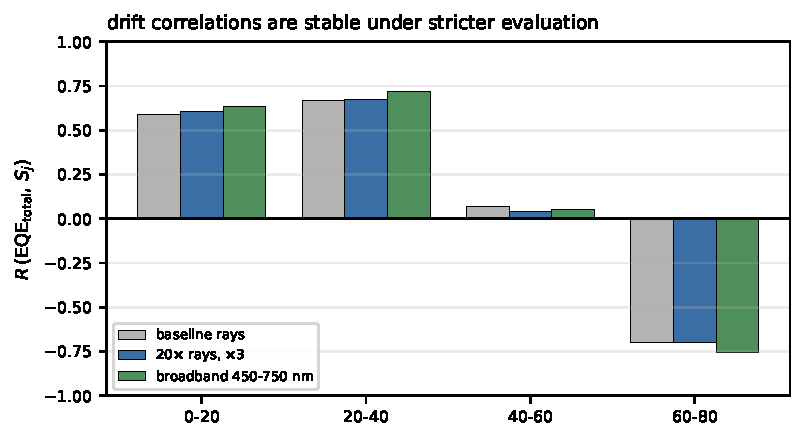
\includegraphics[width=\linewidth]{figures/figS5_convergence.pdf}
\caption*{\textbf{Fig. S5.} \textbf{Convergence of the drift.} Correlation between total EQE and $S_j$ for the stratified 20-design subset under the three evaluation conditions of Table S7.}
\end{figure}

\section*{Note S6 | Cost calibration for the randomly assembled family}

One fixed geometry (seed 7777, mid-range assembly statistics) was re-evaluated under each setting. Because the reported quantities are ratios, the acceptance criterion is band selectivity. \ensuremath{\Delta} selectivity is the largest absolute deviation from the reference across the four bands, in percentage points.

\begin{table}[htbp]
\centering
\footnotesize
\caption*{Table S8. Cost calibration.}
\resizebox{\linewidth}{!}{\begin{tabular}{llllllllll}
\hline
Setting & lenslets & grid & rays & \ensuremath{\lambda} step & \ensuremath{\lambda} & time (s) & speed-up & EQE & \ensuremath{\Delta} selectivity (pp) \\
\hline
reference & 8 \ensuremath{\times} 8 & 201 & 10,000 & 10 nm & 31 & 777.5 & 1.00 & 0.4975 & — \\
half rays & 8 \ensuremath{\times} 8 & 201 & 5,000 & 10 nm & 31 & 529.3 & 1.47 & 0.4992 & 0.38 \\
coarser \ensuremath{\lambda} & 8 \ensuremath{\times} 8 & 201 & 10,000 & 20 nm & 16 & 446.5 & 1.74 & 0.5012 & 0.66 \\
coarser grid & 8 \ensuremath{\times} 8 & 141 & 10,000 & 10 nm & 31 & 704.6 & 1.10 & 0.5016 & 0.28 \\
fewer lenslets & 6 \ensuremath{\times} 6 & 201 & 10,000 & 10 nm & 31 & 543.3 & 1.43 & 0.4947 & 0.54 \\
\textbf{adopted} & \textbf{6 \ensuremath{\times} 6} & \textbf{141} & \textbf{5,000} & \textbf{20 nm} & \textbf{16} & \textbf{181.0} & \textbf{4.30} & \textbf{0.4950} & \textbf{0.39} \\
\hline
\end{tabular}}
\end{table}

The adopted combination is 4.3\ensuremath{\times} faster and shifts selectivity by 0.39 pp. This equals the Monte-Carlo spread measured by repeating one design (0.5\% relative on total EQE). Two individual reductions exceed 0.5 pp on their own, but their effects do not accumulate. This indicates that the deviations are noise rather than bias. The accuracy columns are exactly reproducible because the seed is fixed. The wall-clock times vary by a few percent with machine load. The supercell carries 6 \ensuremath{\times} 6 lenslets on a 141 \ensuremath{\times} 141 height grid. The disorder correlation length is one lenslet pitch, a sixth of the supercell.

\begin{figure}[htbp]
\centering
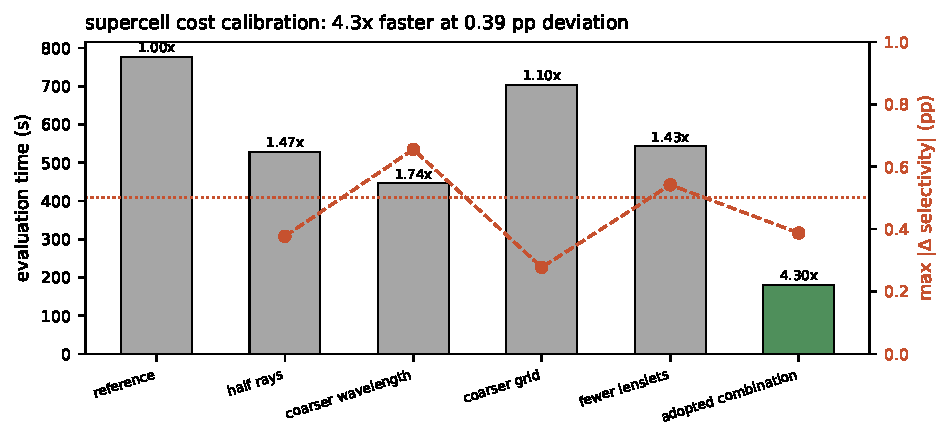
\includegraphics[width=\linewidth]{figures/figS6_cost_calibration.pdf}
\caption*{\textbf{Fig. S6.} \textbf{Supercell cost calibration.} Evaluation time (bars, with speed-up) and largest selectivity deviation from the reference (red markers) for each sampling reduction and for the adopted combination.}
\end{figure}

\section*{Note S7 | Angle-selective light-recycling model}

The calculation behind the recycling route of main-text Table 1 is not a device proposal. It is a reference computation that separates the saturation of non-selective refractive films from the behaviour of selective recycling. We use "light recycling" for the repeated return of reflected substrate light toward the reflective electrode. This avoids confusion with photon recycling by reabsorption and re-emission in the emitter.

\textbf{Model.} The external layer is represented by its angular transmittance $T(\theta,\lambda)$. The reflective electrode and absorption on each round trip are represented by a round-trip loss $a$. A Markov chain tracks the light between the two: at each encounter with the external layer, the transmitted part escapes and the reflected part returns for another attempt, reduced by $a$. The emission of the source into the substrate is taken as Lambertian, and a two-stream scattering layer with asymmetry parameter $g$ may be inserted. With no absorption ($a = 0$) every ray eventually escapes, as in statistical ray optics (main ref. 2). Loss is therefore what limits any recycling scheme.

\textbf{Single-pass wall.} A non-selective layer delivers $\sin^2 60^\circ - \sin^2 40^\circ = 33.7\%$ of the escaping light into the 40–60\ensuremath{^\circ} band (33.8\% numerically). This value is unchanged over $g \in [-0.5, +0.5]$. Without angular selection, recycling only repeats the same partition.

\textbf{Ideal filter.} With $T = 1$ inside the target band and $T = 0$ outside, delivery into the 40–60\ensuremath{^\circ} band reaches 100\% of generated power at $a = 0$. It falls to 62.1\% at $a = 10\%$, whereas the planar non-selective reference stays at 29.1\%. The two converge as $a$ grows, so loss, not filter quality, sets the practical ceiling.

\textbf{Realizable filter.} A transfer-matrix calculation of an alternating high/low-index dielectric multilayer (eight pairs) gives 48.2\% for a monochromatic source. Delivery falls to 32.5\% over a 100 nm source bandwidth, back below the single-pass wall. Source bandwidth is therefore the second practical constraint.

\begin{figure}[htbp]
\centering
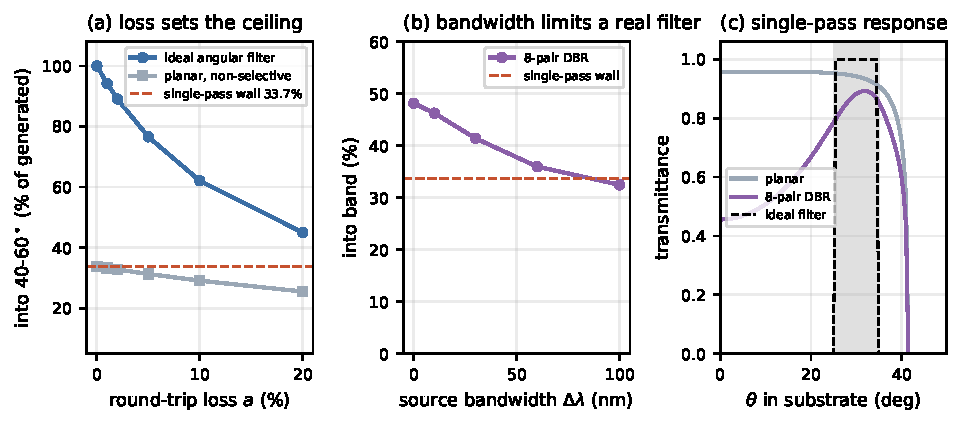
\includegraphics[width=\linewidth]{figures/figS7_recycling_model.pdf}
\caption*{\textbf{Fig. S7.} \textbf{Angle-selective light-recycling model.} (a) Power delivered into the 40–60\ensuremath{^\circ} band, as a fraction of generated power, versus round-trip loss $a$, for the ideal angular filter and the planar non-selective reference; the dashed line is the single-pass wall. (b) Band delivery of the eight-pair dielectric multilayer versus source bandwidth. (c) Single-pass angular transmittance in the substrate of the planar interface, the multilayer, and the ideal filter, with the target band shaded.}
\end{figure}

\section*{Note S8 | Asymmetric three-dimensional freeform exploration}

To check whether axial symmetry itself limits the outcome, three-dimensional asymmetric freeform lenslets were optimized directly against a restricted $(\theta,\phi)$ window, with the objective

\begin{equation*}
\mathrm{EQE}_{\mathrm{win}}=\int_{\theta_1}^{\theta_2}\!\!\int_{\phi_1}^{\phi_2} I_{\mathrm{air}}(\theta,\phi)\,\sin\theta\,d\phi\,d\theta .
\end{equation*}

This was a separate, differently constrained study. It used a different OLED stack (Ag rather than ITO electrode), an anisotropic emitter cell, and 52 shape variables rather than 13. It is therefore not part of the same-constraints benchmark.

The asymmetric shapes could shift the centroid and fine structure of the far field. They did not reliably achieve an absolute window power appreciably above the hemispherical MLA. We report this comparison qualitatively and give no ratio. The stack, emitter cell, and parameter count all differ from the controlled benchmark, so a numerical gain would invite a side-by-side reading that the scope does not support. What carries over is the sign of the effect, not its magnitude. Periodic arrays can steer light under other conditions: asymmetric prisms, diffractive elements, metasurfaces, or sufficient aperture expansion can produce directional emission (main refs. 8, 9). Within coextensive refractive MLAs on a uniform extended source, such redistribution did not become a useful output channel beyond the hemispherical reference.

\section*{Reproducing the figures and data}

All main-text figures are produced by \texttt{make\_figures.py}. The supplementary figures and the raw-data workbooks are produced by \texttt{make\_supp\_figures\_and\_data.py}. Run both from the repository root, in this order:

\begin{verbatim}
python3 make_figures.py
python3 make_supp_figures_and_data.py
\end{verbatim}

The first script reads only the archived result files, prints every number quoted in the captions to \texttt{figure\_numbers.txt}, and writes each figure as PNG (300 dpi) and PDF. The second exports an Excel workbook for every figure, main and supplementary, named after the figure (e.g. \texttt{fig2\_hemisphere\_benchmark.xlsx} alongside \texttt{fig2\_hemisphere\_benchmark.png}). Each workbook has one sheet per panel with exactly the plotted arrays, so any figure can be re-plotted or restyled without the \texttt{.mat} archives. The export script imports the plotting script, so the workbooks cannot drift from the figures.

\begin{table}[htbp]
\centering
\footnotesize
\caption*{Table S9. Figure files and their inputs.}
\begin{tabular}{p{0.16\linewidth}p{0.40\linewidth}p{0.40\linewidth}}
\hline
Figure & Output & Inputs \\
\hline
Fig. 1 & \texttt{fig1\_platform} & \texttt{opt\_4band\_result\_25by25.mat}, \texttt{opt\_hemisphere\_result.mat} \\
Fig. 2 & \texttt{fig2\_hemisphere\_benchmark} & \texttt{opt\_4band\_result\_25by25.mat}, \texttt{opt\_hemisphere\_result.mat}, \texttt{warmstart\_hemisphere\_result.mat}, \texttt{freeform\_EQEtotal\_result.mat} \\
Fig. 3 & \texttt{fig3\_efficiency\_composition} & \texttt{pareto\_front\_result.mat}, \texttt{opt\_4band\_result\_25by25.mat} \\
Fig. 4 & \texttt{fig4\_families} & \texttt{opt\_4band\_result\_25by25.mat}, \texttt{opt\_4band\_inverted\_result.mat}, \texttt{stress\_random\_result.mat} \\
Fig. S1 & \texttt{figS1\_restart\_control} & \texttt{warmstart\_hemisphere\_result.mat}, \texttt{reeval\_confirm\_2040\_result.mat} \\
Fig. S2 & \texttt{figS2\_patch\_dependence} & \texttt{patch\_convergence\_result.mat}, \texttt{patch\_convergence\_100.mat} \\
Fig. S3 & \texttt{figS3\_gain\_decomposition} & \texttt{pareto\_front\_result.mat}, \texttt{opt\_4band\_result\_25by25.mat} \\
Fig. S4 & \texttt{figS4\_selectivity\_map} & \texttt{pareto\_front\_result.mat} \\
Fig. S5 & \texttt{figS5\_convergence} & \texttt{convergence\_check\_result.mat} \\
Fig. S6 & \texttt{figS6\_cost\_calibration} & \texttt{calibrate\_random\_cost.mat} \\
Fig. S7 & \texttt{figS7\_recycling\_model} & \texttt{angular\_recycling\_result.npz}, \texttt{angular\_recycling\_bandwidth.npz} \\
\hline
\end{tabular}
\end{table}

Each output exists as \texttt{.png}, \texttt{.pdf}, and \texttt{.xlsx}.

Result archives: \texttt{pareto\_front\_result.mat}, \texttt{opt\_4band\_result\_25by25.mat}, \texttt{freeform\_EQEtotal\_result.mat}, \texttt{opt\_hemisphere\_result.mat}, \texttt{opt\_4band\_inverted\_result.mat}, \texttt{stress\_random\_result.mat}, \texttt{calibrate\_random\_cost.mat}, \texttt{warmstart\_hemisphere\_result.mat}, \texttt{reeval\_confirm\_2040\_result.mat}, \texttt{patch\_convergence\_result.mat}, \texttt{patch\_convergence\_100.mat}, \texttt{convergence\_check\_result.mat}, \texttt{angular\_recycling\_result.npz}, \texttt{angular\_recycling\_bandwidth.npz}.

\end{document}